\documentclass[12pt]{article}

\usepackage{geometry}
\usepackage{color}
\usepackage{amsmath}
\usepackage{graphicx}
\usepackage{hyperref}

\geometry{
  a4paper,
  right=1.5cm,
  left=1.5cm,
  top=2cm,
  bottom=1.5cm,
}

\begin{document}
 \section{\Huge \color{red} Problem Description}
 
 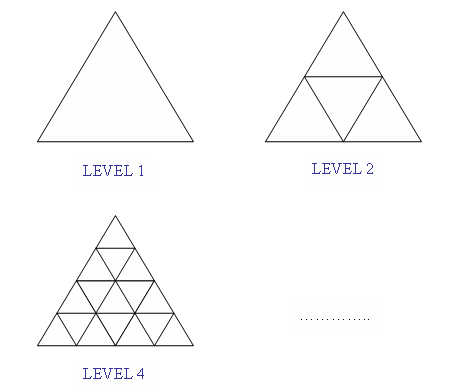
\includegraphics{diag}
 
 \textbf{Count the number of triangles in the triangle of level n.}
 
 \section{\Huge \color{red} My derivation}
 
 Help (Particularly for downward triangles) taken from \url{http://www.math.ku.dk/~mel/mel.pdf}
 
 \subsection{\color{blue}Upward Triangles}
 
 Triangles of level 1 inside the input triangle = 1 + 2 + 3 + 4 + ... + n-3 + n-2 + n-1 + n\\
 Triangles of level 2 inside the input triangle = 1 + 2 + 3 + 4 + ... + n-3 + n-2 + n-1\\
 Triangles of level 3 inside the input triangle = 1 + 2 + 3 + 4 + ... + n-3 + n-2
 \\ \\
 In general,
 
 Triangles of level i in triangle of level n = 1 + 2 + 3 + .... + (n+1-i) = $\displaystyle\frac{(n+1-i)(n+2-i)}{2}$
 
 Summing it for all levels
 
 $\displaystyle\sum_{i=1}^{n} \frac{(n+1-i)(n+2-i)}{2}$
 \\ \\ \\
 $\displaystyle= \frac{(n+1)(n+2)}{2} \displaystyle\sum_{i=1}^{n} (1) - \frac{2n+3}{2} \displaystyle\sum_{i=1}^{n} (i) + \frac{1}{2} \displaystyle\sum_{i=1}^{n} (i^{2})$
 \\ \\ \\
 $\displaystyle= \frac{n(n+1)(n+2)}{2} - \frac{n(n+1)(2n+1)}{4} + \frac{n(n+1)(2n+1)}{12} $
 \\ \\ \\
 $\displaystyle= \frac{n(n+1)}{2}\bigg(n+2 - \frac{2n+3}{2} + \frac{2n+1}{6}\bigg)$
 \\ \\ \\
 $\displaystyle= \frac{n(n+1)(n+2)}{6}$
 \\ \\ \\
 \begin{equation}\label{eq:up}
  = \binom{n+2}{3}
 \end{equation}

 \subsection{\color{blue}Downward Triangles}
 
 Triangle of level i starts from level 2i. \\
 In general,
 Triangles of level i in triangle of level n = 1 + 2 + 3 + ... + (n+1-2i)\\ \\ = $\displaystyle\frac{(n+1-2i)(n+2-2i)}{2}$ \\
 \\ \\
 Also, the maximum level of inverse triangle = $\displaystyle \left \lfloor {\frac{n}{2}}\right \rfloor $
 \\ \\
 Summing it for all levels
 \\ \\ \\
 $\displaystyle\sum_{i=1}^{ \left \lfloor {\frac{n}{2}}\right \rfloor } \frac{(n+1-2i)(n+2-2i)}{2}$ 
 \\ \\ \\
 $\displaystyle= \frac{(n+1)(n+2)}{2} \displaystyle\sum_{i=1}^{\left \lfloor {\frac{n}{2}}\right \rfloor} (1) - (2n+3) \displaystyle\sum_{i=1}^{\left \lfloor {\frac{n}{2}}\right \rfloor} (i) + 2 \displaystyle\sum_{i=1}^{\left \lfloor {\frac{n}{2}}\right \rfloor} (i^{2})$
 \\ \\ \\
 $\displaystyle= \frac{(n+1)(n+2)}{2} \left \lfloor {\frac{n}{2}}\right \rfloor - \frac{2n+3}{2} \left \lfloor {\frac{n}{2}}\right \rfloor \bigg(\left \lfloor {\frac{n}{2}}\right \rfloor + 1 \bigg) + \frac{1}{3} \left \lfloor {\frac{n}{2}}\right \rfloor \bigg(\left \lfloor {\frac{n}{2}}\right \rfloor + 1 \bigg)\bigg(2\left \lfloor {\frac{n}{2}}\right \rfloor+1\bigg) $
 \\ \\ \\
 $\displaystyle= \left \lfloor {\frac{n}{2}}\right \rfloor \Bigg( \frac{(n+1)(n+2)}{2} + \bigg(\left \lfloor {\frac{n}{2}}\right \rfloor + 1 \bigg)\bigg(\frac{2}{3}\left \lfloor {\frac{n}{2}}\right \rfloor+\frac{1}{3} - \frac{2n+3}{2}\bigg)\Bigg)$
 \\ \\ \\
 Replace $\displaystyle\left \lfloor {\frac{n}{2}}\right \rfloor$ by $\displaystyle\frac{n-\delta(n)}{2}$
 \\ \\ 
 On solving, we get
 \\ \\
 $\displaystyle= \frac{2n^{3}+3n^{2}-2n-3\delta(n)}{24}$
 \\ \\
 \begin{equation}\label{eq:down}
  = \frac{2n^{3}+3n^{2}-2n}{24}-\frac{\delta(n)}{8}
 \end{equation}
 \\ \\
 Where we have used the fact that $\delta(n)^{2}=\delta(n)$
 
 \subsection{\color{blue} Total Number of triangles}
 On combining equations \ref{eq:up} and \ref{eq:down} 
 \\ \\
 Total Number of triangles = $\displaystyle\frac{n(n+2)(2n+1)-\delta(n)}{8}$ or $\displaystyle\left \lfloor {\frac{n(n+2)(2n+1)}{8}}\right \rfloor$
 \end{document}
